\sourcepageanchor{112}
\subsection{连续分布}\label{sec:3.3}
本节讨论一些更常见的、有熟悉名称的连续分布族. 这里提到的分布绝不涵盖统计学中使用的所有分布. 实际上，如\autoref{sec:1.6}所见，任何非负、可积的函数都可变换成一个pdf.

\paragraph{均匀分布.}
把质量均匀分布在区间$[a,b]$上，就定义了连续均匀分布（uniform distribution）. 它的pdf为
\begin{equation}\label{eq:3.3.1}\index{SI0387@均匀}
f(x\mid a,b)=\begin{cases}\dfrac1{b-a},&x\in[a,b],\\0,&\text{其他情形}.\end{cases}
\end{equation}
容易验证$\int_a^b f(x)\,dx=1$. 还有
\begin{align*}
EX&=\int_a^b\frac{x}{b-a}\,dx=\frac{b+a}2,\\
\operatorname{Var}X&=\int_a^b\frac{(x-\frac{b+a}2)^2}{b-a}\,dx=\frac{(b-a)^2}{12}.
\end{align*}

\paragraph{Gamma分布.}
Gamma分布族是$[0,\infty)$上一个灵活的分布族，可用\autoref{sec:1.6}讨论的构造方法导出. 若$\alpha$为正常数，则积分
$$\int_0^\infty t^{\alpha-1}e^{-t}\,dt$$
有限. 若$\alpha$为正整数，该积分可用闭式表示，否则不能.\footnote{译注：原文“否则不能”过于绝对；例如本页随后即指出$\Gamma(1/2)=\sqrt\pi$，再由递推关系可得所有正半整数处的闭式值. 此处保留原文表述.} 无论哪种情形，它的值都定义了Gamma函数（gamma function），
\begin{equation}\label{eq:3.3.2}\index{SI0450@伽马函数（另见分布：伽马）}
\Gamma(\alpha)=\int_0^\infty t^{\alpha-1}e^{-t}\,dt.
\end{equation}
Gamma函数满足许多有用的关系，特别是
\begin{equation}\label{eq:3.3.3}
\Gamma(\alpha+1)=\alpha\Gamma(\alpha),\qquad\alpha>0,
\end{equation}
这可用分部积分验证. 结合\eqref{eq:3.3.3}与容易验证的事实$\Gamma(1)=1$，对任意整数$n>0$有
\begin{equation}\label{eq:3.3.4}
\Gamma(n)=(n-1)!.
\end{equation}
（另一个有用的特例是$\Gamma(1/2)=\sqrt\pi$，将在\eqref{eq:3.3.15}中看到.）

\eqref{eq:3.3.3}和\eqref{eq:3.3.4}给出的递推关系，使Gamma函数值的计算更为容易. 借助递推关系，只须知道$\Gamma(c)$在$0<c\le1$时的值，就能计算Gamma函数的任意值.

由于\eqref{eq:3.3.2}中的被积函数为正，立即得到
\begin{equation}\label{eq:3.3.5}
f(t)=\frac{t^{\alpha-1}e^{-t}}{\Gamma(\alpha)},\qquad0<t<\infty
\end{equation}
是一个pdf. 不过，完整的Gamma族具有两个参数. 取正常数$\beta$，在\eqref{eq:3.3.5}中作变量变换，求出随机变量$X=\beta T$的pdf，就得到Gamma$(\alpha,\beta)$族：
\begin{equation}\label{eq:3.3.6}\index{SI0306@伽马}
f(x\mid\alpha,\beta)=\frac1{\Gamma(\alpha)\beta^\alpha}x^{\alpha-1}e^{-x/\beta},\qquad0<x<\infty,\quad\alpha>0,\quad\beta>0.
\end{equation}
\sourcepageanchor{113}

参数$\alpha$称为形状参数（shape parameter），因为它主要影响分布峰的形状；参数$\beta$称为尺度参数（scale parameter），因为它主要影响分布的离散程度.

Gamma$(\alpha,\beta)$分布的均值为
\begin{equation}\label{eq:3.3.7}
EX=\frac1{\Gamma(\alpha)\beta^\alpha}\int_0^\infty xx^{\alpha-1}e^{-x/\beta}\,dx.
\end{equation}
为计算\eqref{eq:3.3.7}，注意被积函数是Gamma$(\alpha+1,\beta)$的pdf的核. 由\eqref{eq:3.3.6}知道，对任意$\alpha,\beta>0$，
\begin{equation}\label{eq:3.3.8}
\int_0^\infty x^{\alpha-1}e^{-x/\beta}\,dx=\Gamma(\alpha)\beta^\alpha,
\end{equation}
所以
\begin{align*}
EX&=\frac1{\Gamma(\alpha)\beta^\alpha}\int_0^\infty x^\alpha e^{-x/\beta}\,dx\\
&=\frac1{\Gamma(\alpha)\beta^\alpha}\Gamma(\alpha+1)\beta^{\alpha+1}\\
&=\frac{\alpha\Gamma(\alpha)\beta}{\Gamma(\alpha)}\qquad(\text{由\eqref{eq:3.3.3}})\\
&=\alpha\beta.
\end{align*}
注意，计算$EX$时，我们再次使用了把积分中的函数识别为另一个pdf的核这一技巧. （此前已用此技巧在\autoref{ex:2.3.8}中计算Gamma矩母函数，并在离散情形下于\autoref{ex:2.2.3}和\autoref{ex:2.3.5}中进行二项分布的计算.）

Gamma$(\alpha,\beta)$分布方差的计算方法类似于均值. 特别地，计算$EX^2$时处理的是Gamma$(\alpha+2,\beta)$分布的核. 结果为
$$\operatorname{Var}X=\alpha\beta^2.$$
在\autoref{ex:2.3.8}中，我们算出了Gamma$(\alpha,\beta)$分布的矩母函数：
$$M_X(t)=\left(\frac1{1-\beta t}\right)^\alpha,\qquad t<\frac1\beta.$$

\begin{example}[Gamma与Poisson的关系]\label{ex:3.3.1}\index{SI0315@与泊松的关系}\index{SI0377@与伽马的关系}
Gamma分布与Poisson分布之间有一个有趣的关系. 若$X$是Gamma$(\alpha,\beta)$随机变量，其中$\alpha$为整数，则对任意$x$，
\begin{equation}\label{eq:3.3.9}
P(X\le x)=P(Y\ge\alpha),
\end{equation}
其中$Y\sim\operatorname{Poisson}(x/\beta)$. 连续使用分部积分可证明\eqref{eq:3.3.9}，如下所示. 因为$\alpha$为整数，写$\Gamma(\alpha)=(\alpha-1)!$，得到
\begin{align*}
P(X\le x)&=\frac1{(\alpha-1)!\beta^\alpha}\int_0^x t^{\alpha-1}e^{-t/\beta}\,dt\\
&=\frac1{(\alpha-1)!\beta^\alpha}\left[\left.-t^{\alpha-1}\beta e^{-t/\beta}\right|_0^x+\int_0^x(\alpha-1)t^{\alpha-2}\beta e^{-t/\beta}\,dt\right],
\end{align*}
其中使用分部积分代换$u=t^{\alpha-1}$，$dv=e^{-t/\beta}\,dt$. 继续计算，有
\begin{align*}
P(X\le x)&=\frac{-1}{(\alpha-1)!\beta^{\alpha-1}}x^{\alpha-1}e^{-x/\beta}+\frac1{(\alpha-2)!\beta^{\alpha-1}}\int_0^x t^{\alpha-2}e^{-t/\beta}\,dt\\
&=\frac1{(\alpha-2)!\beta^{\alpha-1}}\int_0^x t^{\alpha-2}e^{-t/\beta}\,dt-P(Y=\alpha-1),
\end{align*}
其中$Y\sim\operatorname{Poisson}(x/\beta)$. 如此继续，就可建立\eqref{eq:3.3.9}. （见\autoref{exercise:3.19}.）
\end{example}
\sourcepageanchor{114}

Gamma分布有若干重要特例. 若令$\alpha=p/2$，其中$p$为整数，并令$\beta=2$，则Gamma的pdf成为
\begin{equation}\label{eq:3.3.10}\index{SI0245@自由度}\index{SI0280@卡方}
f(x\mid p)=\frac1{\Gamma(p/2)2^{p/2}}x^{(p/2)-1}e^{-x/2},\qquad0<x<\infty,
\end{equation}
即具有$p$个自由度的卡方pdf（chi squared pdf with $p$ degrees of freedom）. 卡方分布的均值、方差和矩母函数，都可以利用前面导出的Gamma公式计算.

卡方分布在统计推断中起着重要作用，特别是在从正态分布抽样时. \autoref{sec:5}将详细讨论这一主题.

令$\alpha=1$，就得到Gamma分布的另一个重要特例. 此时
\begin{equation}\label{eq:3.3.11}\index{SI0289@指数}
f(x\mid\beta)=\frac1\beta e^{-x/\beta},\qquad0<x<\infty,
\end{equation}
即尺度参数为$\beta$的指数pdf（exponential pdf）. 它的均值与方差已在\autoref{ex:2.2.2}和\autoref{ex:2.3.3}中计算过.

指数分布可以用来对寿命建模，类似于离散情形中几何分布的用途. 实际上，指数分布也具有几何分布的“无记忆”性质. 若$X\sim\operatorname{exponential}(\beta)$，即pdf由\eqref{eq:3.3.11}给出，则对$s>t\ge0$有\index{SI0293@无记忆性}\semanticindexanchor{293:114}
$$P(X>s\mid X>t)=P(X>s-t),$$
因为
\begin{align*}
P(X>s\mid X>t)&=\frac{P(X>s,X>t)}{P(X>t)}\\
&=\frac{P(X>s)}{P(X>t)}\qquad(\text{因为 }s>t)\\
&=\frac{\int_s^\infty\frac1\beta e^{-x/\beta}\,dx}{\int_t^\infty\frac1\beta e^{-x/\beta}\,dx}
=\frac{e^{-s/\beta}}{e^{-t/\beta}}\\
&=e^{-(s-t)/\beta}=P(X>s-t).
\end{align*}
另一个同时与指数族和Gamma族有关的分布是Weibull分布. 若$X\sim\operatorname{exponential}(\beta)$，则$Y=X^{1/\gamma}$具有Weibull$(\gamma,\beta)$分布：
\begin{equation}\label{eq:3.3.12}\index{SI0391@威布尔}
f_Y(y\mid\gamma,\beta)=\frac\gamma\beta y^{\gamma-1}e^{-y^\gamma/\beta},\quad0<y<\infty,\quad\gamma>0,\quad\beta>0.
\end{equation}
显然，我们也可以从Weibull分布出发，再把指数分布作为特例（$\gamma=1$）推导出来. 这只是取舍偏好的问题. Weibull分布在失效时间数据分析中起着极为重要的作用［这一主题的全面论述见\hyperref[bib:source186]{Kalbfleisch和Prentice（1980）}］. 特别地，Weibull分布非常适合对风险函数（hazard function）建模［见\autoref{exercise:3.25}和\autoref{exercise:3.26}］.\index{SI0469@风险率函数}\semanticindexanchor{469:114}

\paragraph{正态分布.}\index{SI0317@高斯}\semanticindexanchor{317:114}\index{SI0358@正态}\semanticindexanchor{358:114}
正态分布（normal distribution，有时称为Gaussian分布）在统计学的大量内容中起着核心作用. 主要有三个原因. 第一，正态分布及与它相关的分布非常便于解析处理（虽然乍看之下可能并非如此）. 第二，正态分布具有熟悉的钟形，其对称性使它成为许多总体模型中颇有吸引力的选择. 尽管还有许多其他分布也呈钟形，
\sourcepageanchor{115}
其中大多数却没有正态分布那样便于解析处理. 第三，存在中心极限定理（Central Limit Theorem，详见\autoref{sec:5}）；它表明，在温和条件下，可以在大样本中用正态分布近似种类繁多的分布.

正态分布有两个参数，通常记作$\mu$和$\sigma^2$，它们分别是均值与方差. 均值为$\mu$、方差为$\sigma^2$的正态分布（通常记作$\operatorname n(\mu,\sigma^2)$）的pdf为
\begin{equation}\label{eq:3.3.13}
f(x\mid\mu,\sigma^2)=\frac1{\sqrt{2\pi}\sigma}e^{-(x-\mu)^2/(2\sigma^2)},\qquad-\infty<x<\infty.
\end{equation}
若$X\sim\operatorname n(\mu,\sigma^2)$，则随机变量$Z=(X-\mu)/\sigma$具有$\operatorname n(0,1)$分布，也称为标准正态分布（standard normal distribution）. 写出以下各式便容易证明：\index{SI0368@标准}\semanticindexanchor{368:115}
\begin{align*}
P(Z\le z)&=P\left(\frac{X-\mu}\sigma\le z\right)=P(X\le z\sigma+\mu)\\
&=\frac1{\sqrt{2\pi}\sigma}\int_{-\infty}^{z\sigma+\mu}e^{-(x-\mu)^2/(2\sigma^2)}\,dx\\
&=\frac1{\sqrt{2\pi}}\int_{-\infty}^z e^{-t^2/2}\,dt\qquad\left(\text{令 }t=\frac{x-\mu}\sigma\right),
\end{align*}
这说明$P(Z\le z)$就是标准正态cdf.

因此，所有正态概率都可以利用标准正态分布计算. 此外，计算期望值时可先在$\operatorname n(0,1)$情形下完成具体运算，再把结果变换到$\operatorname n(\mu,\sigma^2)$情形，从而简化计算. 例如，若$Z\sim\operatorname n(0,1)$，则
$$EZ=\frac1{\sqrt{2\pi}}\int_{-\infty}^\infty ze^{-z^2/2}\,dz=\left.-\frac1{\sqrt{2\pi}}e^{-z^2/2}\right|_{-\infty}^\infty=0,$$
所以若$X\sim\operatorname n(\mu,\sigma^2)$，由\autoref{thm:2.2.5}可得
$$EX=E(\mu+\sigma Z)=\mu+\sigma EZ=\mu.$$
类似地，$\operatorname{Var}Z=1$，再用\autoref{thm:2.3.4}，得到$\operatorname{Var}X=\sigma^2$.

我们尚未证明\eqref{eq:3.3.13}在整个实数轴上的积分等于1. 应用标准化变换，只须证明
$$\frac1{\sqrt{2\pi}}\int_{-\infty}^\infty e^{-z^2/2}\,dz=1.$$
注意，上面的被积函数关于0对称，故在$(-\infty,0)$上的积分等于在$(0,\infty)$上的积分. 因此，问题归结为证明
\begin{equation}\label{eq:3.3.14}
\int_0^\infty e^{-z^2/2}\,dz=\frac{\sqrt{2\pi}}2=\sqrt{\frac\pi2}.
\end{equation}
函数$e^{-z^2/2}$没有可用初等函数显式表示（即以闭式表示）的原函数，所以我们不能直接积分. 事实上，这是一类积分的例子：要么你知道怎样做，要么可能花很长时间仍毫无进展. 因为\eqref{eq:3.3.14}的两边都为正，只要证明它们的平方相等，就能得到该等式. 对\eqref{eq:3.3.14}中的积分取平方，得到
\begin{align*}
\left(\int_0^\infty e^{-z^2/2}\,dz\right)^2
&=\left(\int_0^\infty e^{-t^2/2}\,dt\right)\left(\int_0^\infty e^{-u^2/2}\,du\right)\\
&=\int_0^\infty\int_0^\infty e^{-(t^2+u^2)/2}\,dt\,du.
\end{align*}
\sourcepageanchor{116}

积分变量只是哑变量，所以可以改变它们的名称. 现在转为极坐标. 定义
$$t=r\cos\theta\qquad\text{及}\qquad u=r\sin\theta.$$
则$t^2+u^2=r^2$，且$dt\,du=r\,d\theta\,dr$，积分范围变为$0<r<\infty$，$0<\theta<\pi/2$（因为$t$和$u$均限制为正，所以$\theta$的上限为$\pi/2$）. 于是
\begin{align*}
\int_0^\infty\int_0^\infty e^{-(t^2+u^2)/2}\,dt\,du
&=\int_0^\infty\int_0^{\pi/2}re^{-r^2/2}\,d\theta\,dr\\
&=\frac\pi2\int_0^\infty re^{-r^2/2}\,dr
=\frac\pi2\left[\left.-e^{-r^2/2}\right|_0^\infty\right]=\frac\pi2,
\end{align*}
从而证明了\eqref{eq:3.3.14}.

这个积分与Gamma函数密切相关；事实上，在\eqref{eq:3.3.14}中作代换$w=\frac12z^2$，就会看到该积分实质上就是$\Gamma(1/2)$. 如果仔细处理常数，就会看出\eqref{eq:3.3.14}蕴含
\begin{equation}\label{eq:3.3.15}
\Gamma\left(\frac12\right)=\int_0^\infty w^{-1/2}e^{-w}\,dw=\sqrt\pi.
\end{equation}
正态分布在以下意义上有些特殊：它的两个参数$\mu$（均值）和$\sigma^2$（方差）提供了有关分布确切形状与位置的全部信息. 分布由$\mu$和$\sigma^2$确定这一性质，并非正态pdf所独有，而是一族称为位置—尺度族（location--scale families）的pdf所共有的性质；将在\autoref{sec:3.5}讨论.

直接作微积分运算可知，正态pdf \eqref{eq:3.3.13}在$x=\mu$处取最大值，在$\mu\pm\sigma$处有拐点（曲线由凹变凸的位置）. 此外，离均值1、2或3个标准差以内的概率为
\begin{align*}
P(|X-\mu|\le\sigma)&=P(|Z|\le1)=.6826,\\
P(|X-\mu|\le2\sigma)&=P(|Z|\le2)=.9544,\\
P(|X-\mu|\le3\sigma)&=P(|Z|\le3)=.9974,
\end{align*}
其中$X\sim\operatorname n(\mu,\sigma^2)$，$Z\sim\operatorname n(0,1)$，这些数值可由许多计算机软件包或数表得到. 通常报告的两位小数值分别为$.68$、$.95$和$.99$. 尽管这些并非四舍五入值，却是常用的数值. \autoref{fig:3.3.1}展示了正态pdf及这些关键特征.

在正态分布的众多应用中，一个重要应用是近似其他分布（中心极限定理为此提供了部分依据）. 例如，若$X\sim\operatorname{binomial}(n,p)$，则$EX=np$且$\operatorname{Var}X=np(1-p)$；在适当条件下，$X$的分布可用均值$\mu=np$、方差$\sigma^2=np(1-p)$的正态随机变量的分布近似. “适当条件”是$n$应很大，且$p$不应过于极端（接近0或1）. 我们希望$n$足够大，使$X$有足够多的（离散）取值，从而用连续分布近似是合理的；而$p$应处于“中间”，使二项分布像正态分布一样近乎对称. 与大多数近似一样，这里没有绝对准则，每次应用都应检查近似是否足以满足预定用途. 一个保守的经验规则是：若$\min(np,n(1-p))\ge5$，则近似较好.
\sourcepageanchor{117}

\begin{figure}[htbp]
\centering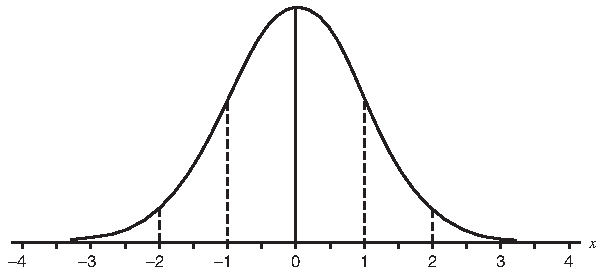
\includegraphics[width=.72\textwidth]{assets/chapter3/fig3-3-1.pdf}
\caption{标准正态密度}\label{fig:3.3.1}
\end{figure}
\begin{example}[正态近似]\label{ex:3.3.2}\index{SI0059@以正态近似二项}\index{SI0198@连续性校正}
设$X\sim\operatorname{binomial}(25,.6)$. 可用均值$\mu=25(.6)=15$、标准差$\sigma=((25)(.6)(.4))^{1/2}=2.45$的正态随机变量$Y$来近似$X$. 因此，
$$P(X\le13)\approx P(Y\le13)=P\left(Z\le\frac{13-15}{2.45}\right)=P(Z\le-.82)=.206,$$
而精确的二项计算给出
$$P(X\le13)=\sum_{x=0}^{13}\binom{25}{x}(.6)^x(.4)^{25-x}=.267,$$
这表明正态近似还不错，但并不十分出色. 不过，通过“连续性校正”（continuity correction）可大大改善近似. 为了解其原理，请看\autoref{fig:3.3.2}，图中展示了$\operatorname{binomial}(25,.6)$的pmf与$\operatorname n(15,(2.45)^2)$的pdf. 我们以宽为1、高等于概率的条形画出二项pmf. 因而条形面积就给出二项概率. 注意在上面的近似中，近似正态的面积小于二项面积（正态面积是13处直线左边的全部面积，而二项面积包含13处直到13.5的整根条形）. 连续性校正通过给截断点加$1/2$，把这块面积补回去. 所以我们不直接近似$P(X\le13)$，而是近似与它等价的表达式（由于离散性）$P(X\le13.5)$，得到
$$P(X\le13)=P(X\le13.5)\approx P(Y\le13.5)=P(Z\le-.61)=.271,$$
\begin{figure}[htbp]
\centering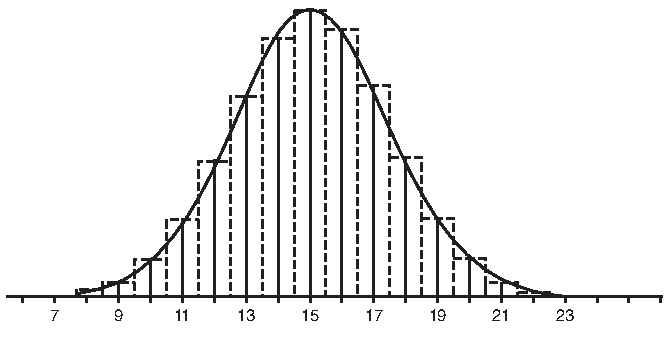
\includegraphics[width=.8\textwidth]{assets/chapter3/fig3-3-2.pdf}
\caption{用正态$(15,(2.45)^2)$近似二项$(25,.6)$}\label{fig:3.3.2}
\end{figure}
\sourcepageanchor{118}
这是好得多的近似. 一般而言，带连续性校正的正态近似远优于没有连续性校正的近似.

下端点也要作校正. 若$X\sim\operatorname{binomial}(n,p)$，$Y\sim\operatorname n(np,np(1-p))$，则我们采用近似
\begin{align*}
P(X\le x)&\approx P(Y\le x+1/2),\\
P(X\ge x)&\approx P(Y\ge x-1/2).
\end{align*}
\end{example}

\paragraph{Beta分布.}
Beta分布族是$(0,1)$上由两个参数标识的连续分布族. Beta$(\alpha,\beta)$的pdf为
\begin{equation}\label{eq:3.3.16}\index{SI0254@贝塔}
f(x\mid\alpha,\beta)=\frac1{B(\alpha,\beta)}x^{\alpha-1}(1-x)^{\beta-1},\quad0<x<1,\quad\alpha>0,\quad\beta>0,
\end{equation}
其中$B(\alpha,\beta)$表示Beta函数（beta function），
$$B(\alpha,\beta)=\int_0^1x^{\alpha-1}(1-x)^{\beta-1}\,dx.$$
Beta函数通过以下恒等式与Gamma函数联系起来：
\begin{equation}\label{eq:3.3.17}\index{SI0089@贝塔函数（另见分布：贝塔）}
B(\alpha,\beta)=\frac{\Gamma(\alpha)\Gamma(\beta)}{\Gamma(\alpha+\beta)}.
\end{equation}
处理Beta函数时，\eqref{eq:3.3.17}非常有用，使我们可以利用Gamma函数的性质. 实际上，我们不会直接处理Beta函数，而会在所有计算中使用\eqref{eq:3.3.17}.

Beta分布是少数几个把概率1赋予一个有限区间的常见“有名”分布之一，这里取的区间是$(0,1)$. 因此，Beta分布常用来对自然位于0与1之间的比例建模. \autoref{sec:4}将给出这方面的例子.

由于pdf的特殊形式，Beta分布的矩很容易计算. 对$n>-\alpha$，有
\begin{align*}
EX^n&=\frac1{B(\alpha,\beta)}\int_0^1x^nx^{\alpha-1}(1-x)^{\beta-1}\,dx\\
&=\frac1{B(\alpha,\beta)}\int_0^1x^{(\alpha+n)-1}(1-x)^{\beta-1}\,dx.
\end{align*}
现在可识别出被积函数是Beta$(\alpha+n,\beta)$的pdf的核，因此
\begin{equation}\label{eq:3.3.18}
EX^n=\frac{B(\alpha+n,\beta)}{B(\alpha,\beta)}=\frac{\Gamma(\alpha+n)\Gamma(\alpha+\beta)}{\Gamma(\alpha+\beta+n)\Gamma(\alpha)}.
\end{equation}
在\eqref{eq:3.3.18}中取$n=1$和$n=2$，并用\eqref{eq:3.3.3}，可算出Beta$(\alpha,\beta)$分布的均值与方差：
$$EX=\frac\alpha{\alpha+\beta}\qquad\text{及}\qquad\operatorname{Var}X=\frac{\alpha\beta}{(\alpha+\beta)^2(\alpha+\beta+1)}.$$
随着参数$\alpha$和$\beta$变化，Beta分布呈现许多形状，如\autoref{fig:3.3.3}所示. pdf可以严格递增（$\alpha>1,\beta=1$）、严格递减（$\alpha=1,\beta>1$）、呈U形（$\alpha<1,\beta<1$）或单峰\mbox{（$\alpha>1,\beta>1$）.} 当$\alpha=\beta$时，pdf关于$1/2$对称，
\sourcepageanchor{119}

\begin{figure}[htbp]
\centering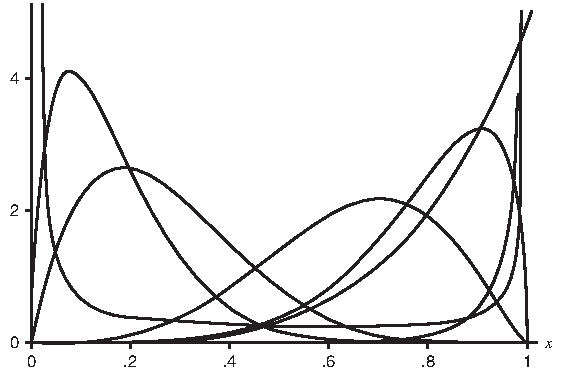
\includegraphics[width=.72\textwidth]{assets/chapter3/fig3-3-3.pdf}
\caption{Beta密度}\label{fig:3.3.3}
\end{figure}
\begin{figure}[htbp]
\centering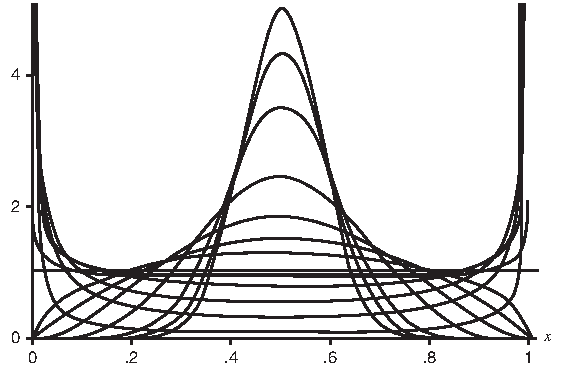
\includegraphics[width=.72\textwidth]{assets/chapter3/fig3-3-4.pdf}
\caption{对称Beta密度}\label{fig:3.3.4}
\end{figure}
其均值（必然）为$1/2$，方差为$(4(2\alpha+1))^{-1}$. 随$\alpha$增加，pdf更集中，但保持对称，如\autoref{fig:3.3.4}所示. 最后，若$\alpha=\beta=1$，Beta分布就化为均匀$(0,1)$分布，说明均匀分布可视为Beta族的成员. Beta分布还通过一个变换与$F$分布相关，后者在统计分析中起着极为重要的作用（见\autoref{sec:5.3}）.

\paragraph{Cauchy分布.}
Cauchy分布是在$(-\infty,\infty)$上对称的钟形分布，其pdf为
\begin{equation}\label{eq:3.3.19}\index{SI0276@柯西}
f(x\mid\theta)=\frac1\pi\frac1{1+(x-\theta)^2},\qquad-\infty<x<\infty,\quad-\infty<\theta<\infty.
\end{equation}
（更一般的Cauchy pdf见\autoref{exercise:3.39}.）从外观上看，Cauchy分布似乎与正态分布没有很大差别. 然而，二者确实有非常大的区别.
\sourcepageanchor{120}

\begin{figure}[htbp]
\centering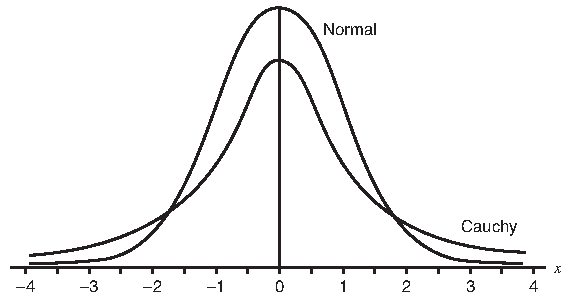
\includegraphics[width=.72\textwidth]{assets/chapter3/fig3-3-5.pdf}
\caption{标准正态密度与Cauchy密度}\label{fig:3.3.5}
\end{figure}
如\autoref{sec:2}中所见，Cauchy分布的均值不存在，即
\begin{equation}\label{eq:3.3.20}
E|X|=\int_{-\infty}^\infty\frac1\pi\frac{|x|}{1+(x-\theta)^2}\,dx=\infty.
\end{equation}
\needspace{5\baselineskip}容易看出，\eqref{eq:3.3.19}对所有$\theta$都定义了一个恰当的pdf. 回顾$\frac d{dt}\arctan(t)=(1+t^2)^{-1}$，因此
$$\int_{-\infty}^\infty\frac1\pi\frac1{1+(x-\theta)^2}\,dx=\left.\frac1\pi\arctan(x-\theta)\right|_{-\infty}^\infty=1,$$
因为$\arctan(\pm\infty)=\pm\pi/2$.

由于$E|X|=\infty$，Cauchy分布的各阶矩都不存在；换言之，所有绝对矩都等于$\infty$.\footnote{译注：此处“各阶矩”“所有绝对矩”应按上下文理解为正整数阶矩；若允许非整数阶，则$0<q<1$时$E|X|^q$有限.} 特别地，矩母函数不存在.

\eqref{eq:3.3.19}中的参数$\theta$确实衡量分布的中心：它是中位数. 若$X$具有参数为$\theta$的Cauchy分布，则由\autoref{exercise:3.37}可得$P(X\ge\theta)=1/2$，这说明$\theta$是分布的中位数. \autoref{fig:3.3.5}把Cauchy$(0)$分布与$\operatorname n(0,1)$分布画在一起；可以看到二者形状相似，但Cauchy的尾部厚得多.

Cauchy分布在统计理论中扮演特殊角色. 它代表一种可用来检验猜想的极端情形. 但不要误以为Cauchy分布只是一个病态例子，因为它会在最意想不到的地方出现. 例如，实验人员经常计算观测值之比，即随机变量之比. （衡量生长时，通常把体重与身高合成一个量——身高对应体重，即体重/身高.）一个令人惊讶的事实是，两个标准正态变量之比具有Cauchy分布（见\autoref{ex:4.3.6}）. 取比值可能导致表现不良的分布.

\paragraph{对数正态分布.}
若随机变量$X$的对数服从正态分布（即$\log X\sim\operatorname n(\mu,\sigma^2)$），则$X$具有对数正态分布（lognormal distribution）. 用\autoref{thm:2.1.5}对正态pdf作直接变换，就得到$X$的pdf：
\begin{equation}\label{eq:3.3.21}\index{SI0332@对数正态}
f(x\mid\mu,\sigma^2)=\frac1{\sqrt{2\pi}\sigma}\frac1x e^{-(\log x-\mu)^2/(2\sigma^2)},\quad0<x<\infty,\quad-\infty<\mu<\infty,\quad\sigma>0,
\end{equation}
\sourcepageanchor{121}

即对数正态pdf. $X$的矩可以直接用\eqref{eq:3.3.21}计算，也可利用与正态分布的关系，写成
\begin{align*}
EX&=Ee^{\log X}=Ee^Y\qquad(Y=\log X\sim\operatorname n(\mu,\sigma^2))\\
&=e^{\mu+(\sigma^2/2)}.
\end{align*}
最后一个等式通过识别正态分布的矩母函数而得到（令$t=1$；见\autoref{exercise:2.33}）. 用类似技巧可计算$EX^2$，得到
$$\operatorname{Var}X=e^{2(\mu+\sigma^2)}-e^{2\mu+\sigma^2}.$$
对数正态分布的外观与Gamma分布相似，如\autoref{fig:3.3.6}所示. 当感兴趣的变量右偏时，这个分布在建模应用中很常见. 例如，收入必然右偏，而用对数正态分布建模，就可以对$\log(\text{收入})$使用正态理论统计方法，这十分方便.

\paragraph{双指数分布.}
把指数分布关于其均值反射，就形成双指数分布（double exponential distribution）.\footnote{译注：原文说“关于其均值反射”；就下面给出的密度而言，准确的构造是以$\mu$为中心，将指数形状的右半支及其镜像各赋予一半质量. 普通指数分布直接关于其自身均值反射，并不会得到此式.} 它的pdf为
\begin{equation}\label{eq:3.3.22}
f(x\mid\mu,\sigma)=\frac1{2\sigma}e^{-|x-\mu|/\sigma},\qquad-\infty<x<\infty,\quad-\infty<\mu<\infty,\quad\sigma>0.
\end{equation}
双指数给出一个具有“肥”尾（比正态尾部肥得多）的对称分布，但它的所有矩仍然存在. 直接计算可得
$$EX=\mu\qquad\text{及}\qquad\operatorname{Var}X=2\sigma^2.$$
双指数分布并非钟形. 事实上，它在$x=\mu$处有一个尖峰（更正式地说，是一个不可微点）. 对这一分布作解析处理时，牢记这一点很重要. 绝对值符号在积分时也可能带来麻烦，最好以$x=\mu$为界把积分分成两个区域：
\begin{equation}\label{eq:3.3.23}\index{SI0288@双指数}
\begin{aligned}
EX&=\int_{-\infty}^\infty\frac{x}{2\sigma}e^{-|x-\mu|/\sigma}\,dx\\
&=\int_{-\infty}^\mu\frac{x}{2\sigma}e^{(x-\mu)/\sigma}\,dx+\int_\mu^\infty\frac{x}{2\sigma}e^{-(x-\mu)/\sigma}\,dx.
\end{aligned}
\end{equation}
注意，在这两个积分区域内可以去掉绝对值符号. （一般而言，这个策略对处理含绝对值的积分很有用：把积分区域分开，使绝对值符号可以去掉.）对每个积分使用分部积分，就可完成\eqref{eq:3.3.23}的计算.

还有许多连续分布可用于不同的统计应用，其中很多会在本书后续内容中出现. \hyperref[bib:source177]{Johnson和Kotz（1969、1970a、1970b）}的综合性著作，是查阅多数常用统计分布的宝贵参考资料.
\sourcepageanchor{122}

\begin{figure}[htbp]
\centering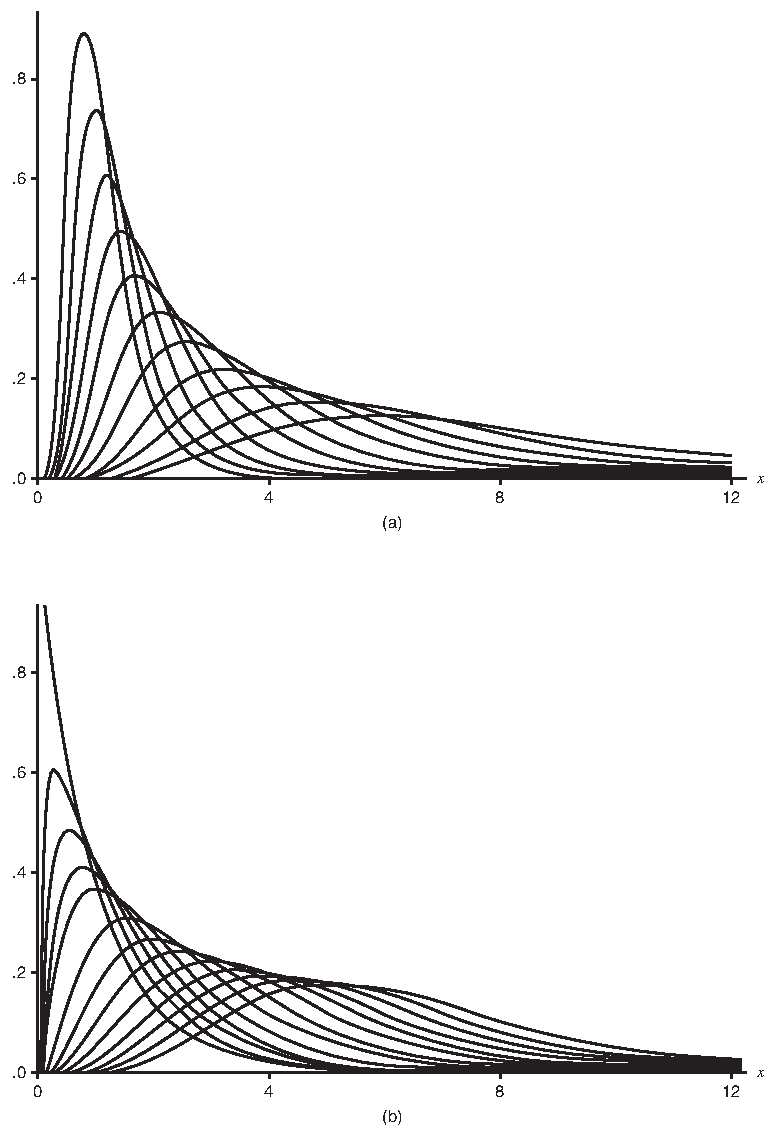
\includegraphics[height=.78\textheight]{assets/chapter3/fig3-3-6.pdf}
\caption{(a)若干对数正态密度；(b)若干Gamma密度}\label{fig:3.3.6}
\end{figure}
